\documentclass[11pt]{article}
\usepackage[T1]{fontenc}
\usepackage[utf8]{inputenc}
\usepackage{lmodern,amsmath,amssymb,graphicx,geometry,microtype,setspace,booktabs,caption}
\usepackage[hidelinks]{hyperref}
\geometry{letterpaper,margin=1in}
\setlength{\parindent}{0pt}
\setlength{\parskip}{0.55em}
\setlength{\emergencystretch}{2em}
\captionsetup{labelfont=bf,font=small}
\renewcommand{\refname}{References}

\pagestyle{empty}
\renewcommand{\thefigure}{S\arabic{figure}}
\setcounter{figure}{0}

\begin{document}
\begin{figure}[!ht]\centering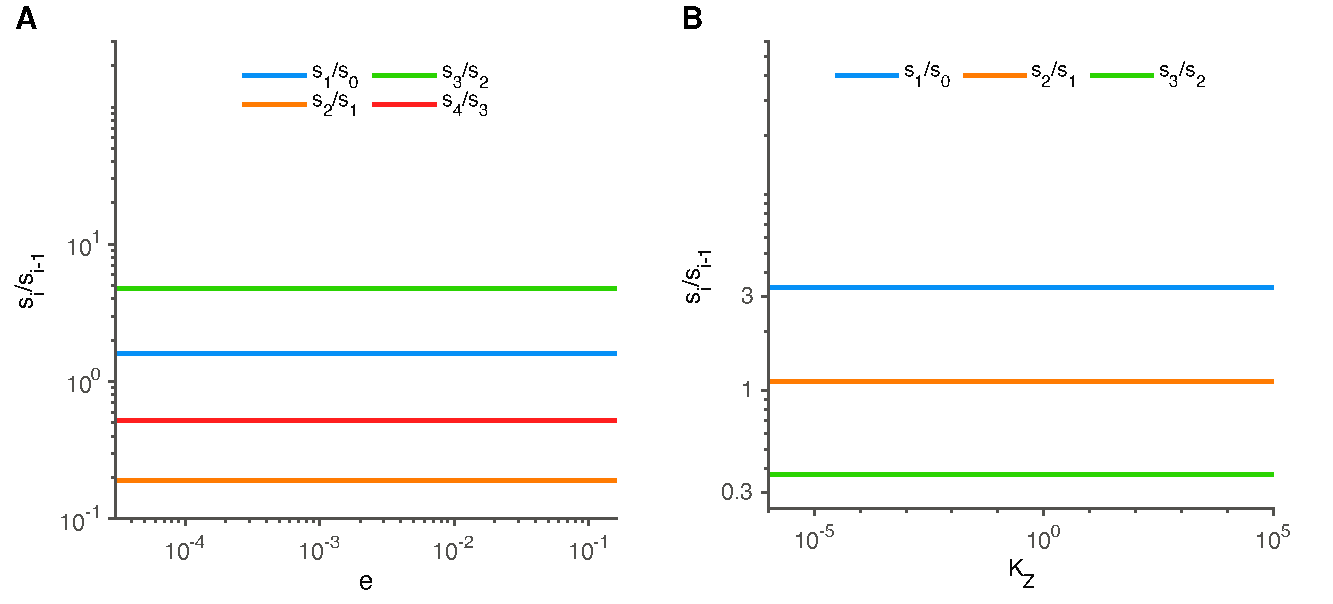
\includegraphics[width=\textwidth,height=0.65\textheight,keepaspectratio]{figure_inputs/FigS1_invariants.pdf}\begin{singlespace}\caption{Numerical checks of the steady-state invariant. (A) Adjacent free-target ratios over a 5,278-fold enzyme sweep at fixed free effector in a four-site nonidentical ladder. (B) A three-site example with a reversible dead end swept over eleven decades at fixed total effector. The small ratio drift reflects the changed free effector; it is not a violation of the free-input identity. See S10 and the source parameter records.}\end{singlespace}\end{figure}
\end{document}
